% !TeX encoding = UTF-8
% !TeX spellcheck = it_IT
% !TeX root = MatDiz.tex
\chapter{J}
\vspace{5mm}
\lemma{Jones William}(1675-1749)Fu il primo ad associare il simbolo $\pi$ al rapporto tra circonferenza e diametro\pointsto~\seeentry{pi greco}.\index{Jones William}
\begin{figure}
	\centering\scaptionb{William Jones (1675 - 1749)}
	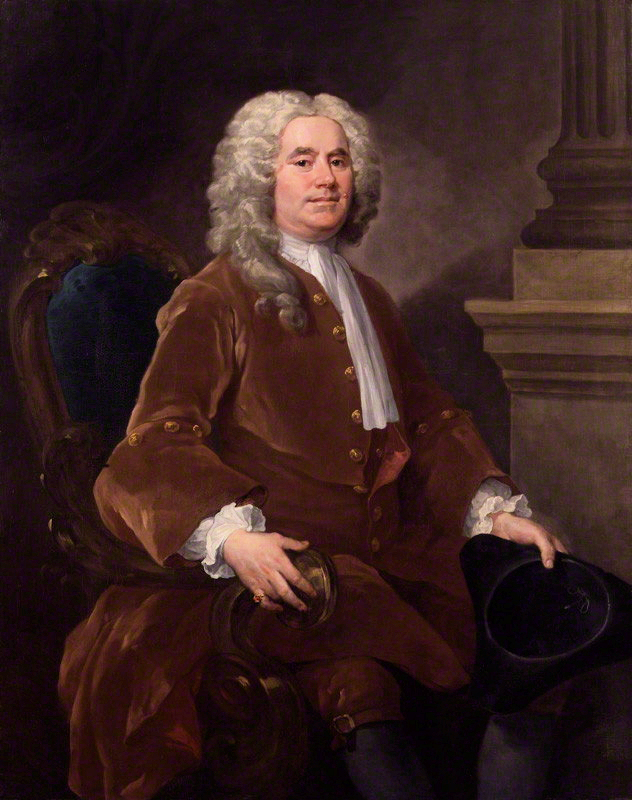
\includegraphics[width=0.7\linewidth]{Figure/J/William_Jones,_the_Mathematician}
		\label{fig:williamjonesthemathematician}
\end{figure}
